% planner_ablation_multifig.tex -- fig_basin_mismatch as two stacked column-width
% subfigures with LaTeX subcaptions, plus the main-body subsection (2026-09-14).
%
% Preamble: \usepackage{subcaption} (after caption, which \captionof already
% loads). The two PDFs are figures/planner/fig_basin_mismatch_{a,b}.pdf, drawn
% by studies/planner_ablation/paper_figs.py (fig_basin_mismatch_split) at the
% geometry of the combined fig_basin_mismatch.pdf, with the panel letters and
% the footnote removed; the captions carry those. Every number is from the
% deploy-gains bench (lean_bench --gains deploy, strategy 25, 33 plans/s and six
% seeds per cell unless stated). The same label fig:planner_basin is used by
% planner_ablation.tex, so \input one file or the other.

\begin{figure}[t]
\centering
\begin{subfigure}{\columnwidth}
  \centering
  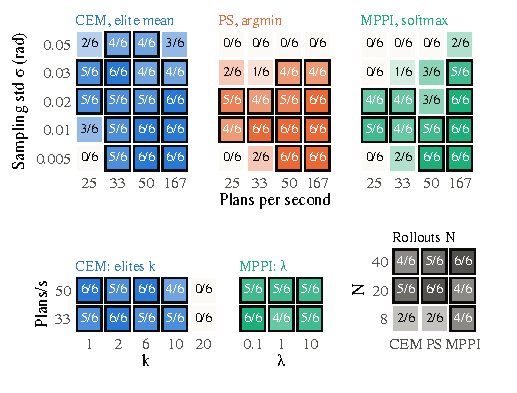
\includegraphics[width=\columnwidth]{figures/planner/fig_basin_mismatch_a.pdf}
  \caption{Configuration. Success rate over sampling standard deviation and plan
  rate for each update rule on the hold spline, and over CEM's elite count $k$,
  MPPI's temperature $\lambda$ and the rollout count $N$ (at 33 plans/s); six
  seeds per cell, outlined at $\ge 4/6$.}
  \label{fig:planner_basin_a}
\end{subfigure}

\vspace{2pt}
\begin{subfigure}{\columnwidth}
  \centering
  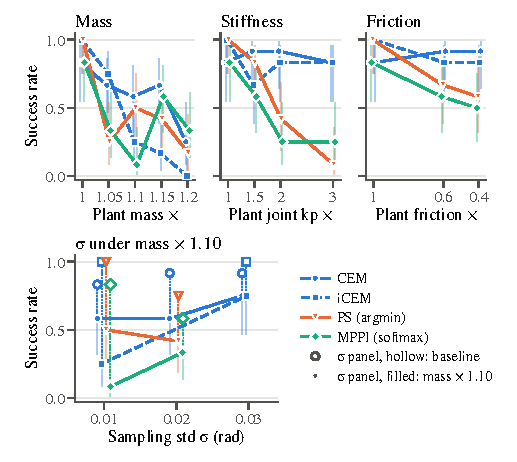
\includegraphics[width=\columnwidth]{figures/planner/fig_basin_mismatch_b.pdf}
  \caption{Model error. Success rate at 33 plans/s when the plant's mass, joint
  stiffness or sliding friction is scaled and the planner's model is not, and
  the same rules with a wider sampling standard deviation at baseline (hollow)
  and under $1.10\times$ mass (filled); 12 seeds, Wilson 95\% intervals.}
  \label{fig:planner_basin_b}
\end{subfigure}
\caption{\textbf{Sampling-based planner ablation: sensitivity to configuration
and to model error.} Hold spline, $\sigma=0.01$\,rad, $N=20$, $k=6$ and
$\lambda=1$ unless varied.}
\label{fig:planner_basin}
\end{figure}

\subsection{Planner Ablation}\label{sec:planner_ablation}
At the robot's joint gains and its 33 plans/s, CEM as shipped in MJPC completes
the ladder (stand, lean, reach, release, four stand-back rungs) on 5/6 seeds
and iCEM on 6/6; predictive sampling (PS) and MPPI complete 0/6, PS falling in
the initial stand on five seeds and MPPI before or during the lean on every
seed. Two of the three components that differ between the planners account for
the gap. PS and MPPI scale their noise by the control range,
$0.12\times\tfrac12\,\mathrm{ctrlrange}=0.03$--$0.36$\,rad per joint (median
$0.21$), where CEM samples in radians with a $0.01$\,rad floor; set to
$0.01$\,rad on the cubic spline MJPC's sampling planner ships with, PS and MPPI
still complete 0/6 and 1/6. With the zero-order hold that CEM hard-codes, PS at
$0.01$\,rad completes 6/6 and MPPI 4/6, and CEM on the cubic spline drops to
1/6: across twenty spline, knot-count and noise-colour configurations, every
one in which the sampled perturbation of the executed action decorrelates
(autocorrelation below $0.8$) within $0.20$\,s of the rollout completes 0--2/6
and every one that holds it to $0.22$\,s completes 5--6/6, for all four
planners. A three-knot hold gives $0.33$\,s by construction; iCEM's AR(1) knot
noise gives it by correlation, which is why iCEM completes with either spline.
The update rule (\textsc{Fold} in Alg.~\ref{alg:skeleton}) is not one of the
two: with the hold and $0.01$\,rad the argmin (PS, and CEM with one elite), the
mean of $k\le 10$ elites and the softmax mean all complete 4--6/6, and only
$k=20$, no selection at all, completes 0/6 (Fig.~\ref{fig:planner_basin}a).

The update rule decides sensitivity instead. Over $\sigma\times$plan rate
(Fig.~\ref{fig:planner_basin}a) CEM completes $\ge 4/6$ in 16 of 20 cells, PS
on the hold in 12, MPPI in 10 and PS on its shipped cubic spline in 5 of 15; at
33 plans/s CEM's admissible $\sigma$ spans the tested decade and the other
rules' one octave. The elite mean's random step is $\sigma/\sqrt{k}$ where the
argmin's is a full $\sigma$, and that is what lets it trade noise for rate: at
$0.01$\,rad every rule needs 25--33 plans/s (16.7 plans/s completes 0--1/6, the
22\,Hz desktop failure of Sec.~\ref{sec:method}), and at $0.02$\,rad CEM
completes 5/6 at 16.7 plans/s where PS and MPPI gain nothing from the same
change. The executed target step per plan depends on $\sigma$ and the rule and
not on the rate (CEM $5$--$8$\,mrad from 167 down to 5 plans/s), so the speed
at which a sampling planner can move its position setpoints is
step\,$\times$\,rate, and the lean onset needs $30$--$40$\,mrad/s of directed
setpoint motion, which 33 plans/s just supplies; the $12$\,s stand survives at
5 plans/s.

The same asymmetry holds against model error (Fig.~\ref{fig:planner_basin}b;
the plant's mass, joint stiffness or sliding friction is scaled after the
planner has taken its model, 12 seeds per cell). Pooled over the three axes
CEM completes 80/108, the argmin 47/108 and the softmax mean 42/108 (one-sided
Fisher $p=4\times10^{-6}$ and $1\times10^{-7}$). A plant two or three times as
stiff as the model costs CEM nothing (11, 10/12) and PS 7--11 seeds, every loss
a fall at the lean onset, where the argmin executes one sample's full step;
friction at $0.4\times$ costs CEM and iCEM nothing and PS and MPPI 5--6 seeds.
Mass is the hard axis for every rule and the one on which iCEM fails (3/12 at
$1.10\times$, every loss a fall in the stand: the heavier plant sags under the
joint PD and iCEM's $3$\,mrad step cannot walk the setpoints out of the sag);
widening its floor to $0.03$\,rad restores 9/12, and the same widening costs
CEM nothing at baseline (11/12) and PS three seeds. This is tolerance to
parametric plant error; estimator noise and unmodelled actuator dynamics are
not in the bench.
